%% uctest.tex 11/3/94
%% Copyright (C) 1988-2004 Daniel Gildea, BBF, Ethan Munson.
%
% This work may be distributed and/or modified under the
% conditions of the LaTeX Project Public License, either version 1.3
% of this license or (at your option) any later version.
% The latest version of this license is in
%   http://www.latex-project.org/lppl.txt
% and version 1.3 or later is part of all distributions of LaTeX
% version 2003/12/01 or later.
%
% This work has the LPPL maintenance status "maintained".
% 
% The Current Maintainer of this work is Daniel Gildea.

\documentclass[11pt]{ucthesis}
\setlength\parindent{0.5cm}

%% The graphicx package provides the includegraphics command.
\usepackage{graphicx}
\graphicspath{{../../../latex/graphics/}{./figures/}{./graphics/}}
%% The amssymb package provides various useful mathematical symbols
\usepackage{amssymb}
\usepackage{amsmath}
\usepackage{amsthm}
\usepackage{relsize} % \mathlarger
\usepackage{mathtools}
\usepackage{braket}
\usepackage{enumerate, enumitem}
\usepackage{caption}
\usepackage{subcaption}
\usepackage{float}

\def\dsp{\def\baselinestretch{2.0}\large\normalsize}
\dsp

\newcommand{\vect}[1]{{\it{\boldsymbol{#1}}}}

\begin{document}
% Declarations for Front Matter

\title{FASTPas - Fast Predictive Aerial Scanning}
\author{Sargis S Yonan}
\degreeyear{2018}
\degreemonth{June}
\degree{MASTER OF SCIENCE}
\chair{Professor Gabriel Hugh Elkaim}
\committeememberone{Professor Numero Dos}
\committeemembertwo{Professor Numero Tres}
\numberofmembers{3} %% (including chair) possible: 3, 4, 5, 6
\deanlineone{Dean Tyrus Miller}
\deanlinetwo{Vice Provost and Dean of Graduate Studies}
\deanlinethree{}
\field{COMPUTER ENGINEERING}
\emphasis{ROBOTICS AND CONTROL}
\campus{Santa Cruz}

\begin{frontmatter}

\maketitle
\copyrightpage

\tableofcontents
\listoffigures
\listoftables

\begin{abstract}

Unmanned Aerial Vehicles (UAVs) have become more prevalent in fields of work and study that benefit from having a birds eye view on a given situation. Firefighter teams have been using UAVs to find the origin of fires, and where fires are spreading to. Scientific researchers have been using aerial thermal imaging to determine rates of change in ice growth and melting, and thermal exchange between the ocean and atmosphere.
\par
The use of autonomous UAVs could benefit rescue teams, firefighters, scientific re- searchers, and private sector industries in the interest of time and data discovery. Using a single or multiple UAVs in a flying network, an area with fields of interest can be scanned efficiently completely autonomously. By simply drawing on a map the general area wished to be scanned by the autonomous fleet, a deployed pod of these UAVs can stream back, to a ground station, live aerial information. This mapping time can be greatly reduced with the use of statistical interpolation techniques that help the pod or single UAV avoid having to scan an entire region, but rather, have the UAVs scan the areas with the lowest level of confidence in prediction.
\par
The Kriging Method, a popular interpolation tool offers a prediction and a variance of prediction, but is computationally expensive because of constant fitting procedures. We can exploit the Kriging variances generated by our prediction to motivate the UAVs to autonomously steer in the areas of least confidence until a minimum confidence in prediction is achieved for an entire unknown field. By designing a computational efficient algorithm based on a Universal Kriging Method, the system is feasible and could benefit a large group of potential users.
\end{abstract}

\begin{dedication}
\null\vfil
{\large
\begin{center}
To all who think flying robots are cool
\vspace{12pt}
\end{center}}
\vfil\null
\end{dedication}


\begin{acknowledgements}
I want to thank Sharon Rabinovich, who reminded me: "Although a cow is tied up, it still wants eat grass."

%who helped me make sense of the various concepts involved in and out of this project. I would like to extend my thanks to the rest of the Autonomous Systems Lab at UC Santa Cruz for the support and motivation to continue this project everyday.
\end{acknowledgements}

\end{frontmatter}

\part{Background}

\section{Mathematical and Geographical Background}
We will exploit several concepts developed in the field of Geostatistics and Geography to assist our flight planning and aerial prediction system. Tobler's First Law of Geography states, "Everything is related to everything else, but near things are more related than distant things."\cite{tobler:first_law} Regarding geospatial data, we can say at the very least, there is a positive correlation between entities that are closely related in distance.\cite{miller:on_toblers_first_law}, implying the existence of spatial autocorrelation in observed geographies. We can exploit this fundamental law of Geography for Geostatistical interpolation methods like inverse distance weighting. Furthermore, if we view our observed fields as an unknown stochastic process, with a generally known model, there exists an overall trend with correlated variation between observed points. We can use these additional caveats to create a Best Linear Unbiased Predictor (BLUP) which can robustly predict intermediate spatial points between observations alongside an additional measure of confidence. We Will exploit these geostatiscal processes to construct graphs of confidence for flight planning, and to predict unknown fields, aerially using UAVs, to some degree of confidence.

\subsection{Measuring and Estimating Points of Interest on a Field}
The basis of our predictions will be observations we make using reliable sensors. For the methods we will explore and develop, we must estimate the coordinates, likely using The Global Positioning System, for each point of interest we measure. In order to use the techniques we will explore we must assume that we can get a Euclidean distance between any two measured points. If a GPS sensor is used to estimate position, we will likely use a Haversine Transformation to convert Earth longitude and latitude estimated by our sensor to points on a Cartesian plane where we will represent our measurements. For each coordinate measured, we will also need to measure some value of interest. If tracking and predicting the current location of a wildfire, for example, we will likely use an infrared sensor to measure the thermal output of the field in which we would like to predict.\\

\subsection{Random Field Notation}
For the sake of convention throughout this work, we will denote $(\vect{x_1}, \vect{x_2})$ to be vectors of position measurements on the domain and co-domain of the Cartesian plane respectively. The $i^{th}$ element of each vector, as a point-pair denoted as $\vect{x}_i = (x_{1_i}, x_{2_i})$, will represent the location of the $i^{th}$ observed location on the Cartesian plane.\\
We will denote the vector, $\vect{u}$, to be a vector of our measured values at our $i^{th}$ observation. The $i^{th}$ element of $\vect{u}$ will correspond to a scalar observation located at $(x_{1_i}, x_{2_i})$, a random variable in a stochastic process, or field, $Z$. Giving us, $Z(\vect{x})=u(\vect{x})$, where $u(\vect{x}): \vect{x} \rightarrow \mathbb{R},\ \vect{x} \in \rm{D} \subset \mathbb{R}^2$\\

\subsection{Autocorrelation in a Field}
Positively correlated geospatial autocorrelation in a field implies the existance of a cluster of similar observed values near one another. The opposite is true when the overall geospatial autocorellation of a field in negative. We can assume, from Tobler's First Law of Geography, that the fields we will measure will contain positive autocorrelation. This degree of geospatial autocorrelation can be measured, and will be discussed in the subsection on variography.

\begin{figure*}[ht!]
    \centering
    \begin{subfigure}[t]{0.5\textwidth}
        \centering
        \includegraphics[width=\linewidth]{figures/generated_field_top_view.png}
        \captionsetup{skip=0.5\baselineskip,size=footnotesize}
        \caption{Top view of the generated field}
		\label{fig:top_view_field}
    \end{subfigure}%
    ~ 
    \begin{subfigure}[t]{0.5\textwidth}
        \centering
        \includegraphics[width=\linewidth]{figures/generated_field_side_view.png}
		\captionsetup{skip=0.5\baselineskip,size=footnotesize}
		\caption{Side view of the generated field}
		\label{fig:side_view_field}
    \end{subfigure}
    \captionsetup{skip=0.5\baselineskip,size=footnotesize}
    \caption{A Gaussian distributed randomly generated spatially autocorrelated field created in MATLAB}
    \label{fig:gen_field}
\end{figure*}

\subsection{Inverse Distance Weighting}
A simple Inverse Distance Weighting (IDW), using Shepard's Method \cite{shepard:idw}, gives us a prediction of observation, $u$, at location $\vect{x}$ to be:
\begin{equation}
	u(\vect{x})=\begin{cases}
			\dfrac{\sum\limits_{i=1}^N w(\vect{x}_i)u_i}{\sum\limits_{i=1}^{N} w(\vect{x}_i)} & \text{if}\ d(\vect{x},\vect{x}_i) \neq 0\ \forall i \\
			u_i & \text{if}\ d(\vect{x},\vect{x}_{i})=0\\
		\end{cases}
\end{equation}\\
where\\
\begin{equation}
	w(\vect{x}_i)=\frac{1}{d(\vect{x},\vect{x}_{i})^{p}}
\end{equation}\\
where, in our cases,\\
\begin{equation}
	d(\vect{x},\vect{x}_{i})^{p} = \|\vect{x}-\vect{x}_i\|_{2}^p
\end{equation}\\
and $p$ is a positive real number, called the power parameter.\\
This method gives us a prediction of all points $\vect{x}$ in a field where a set of observations at labeled positions were made, i.e. $Z(\vect{x})=u(\vect{x})$. Unfortunately, the method is limited in that it does not take advantage of the underlying stochastic model of the field, $Z$, being observed. We will further expand on this method to exploit the fact that $Z$ is a stochastic process with underlying geospatially autocorrelated random variables.\\
In order to apply the Inverse Distance Weighting prediction method to the previously generated map, we will first generate a random set of sample points.

\begin{figure*}[ht!]
    \centering
    \begin{subfigure}[t]{0.5\textwidth}
        \centering
        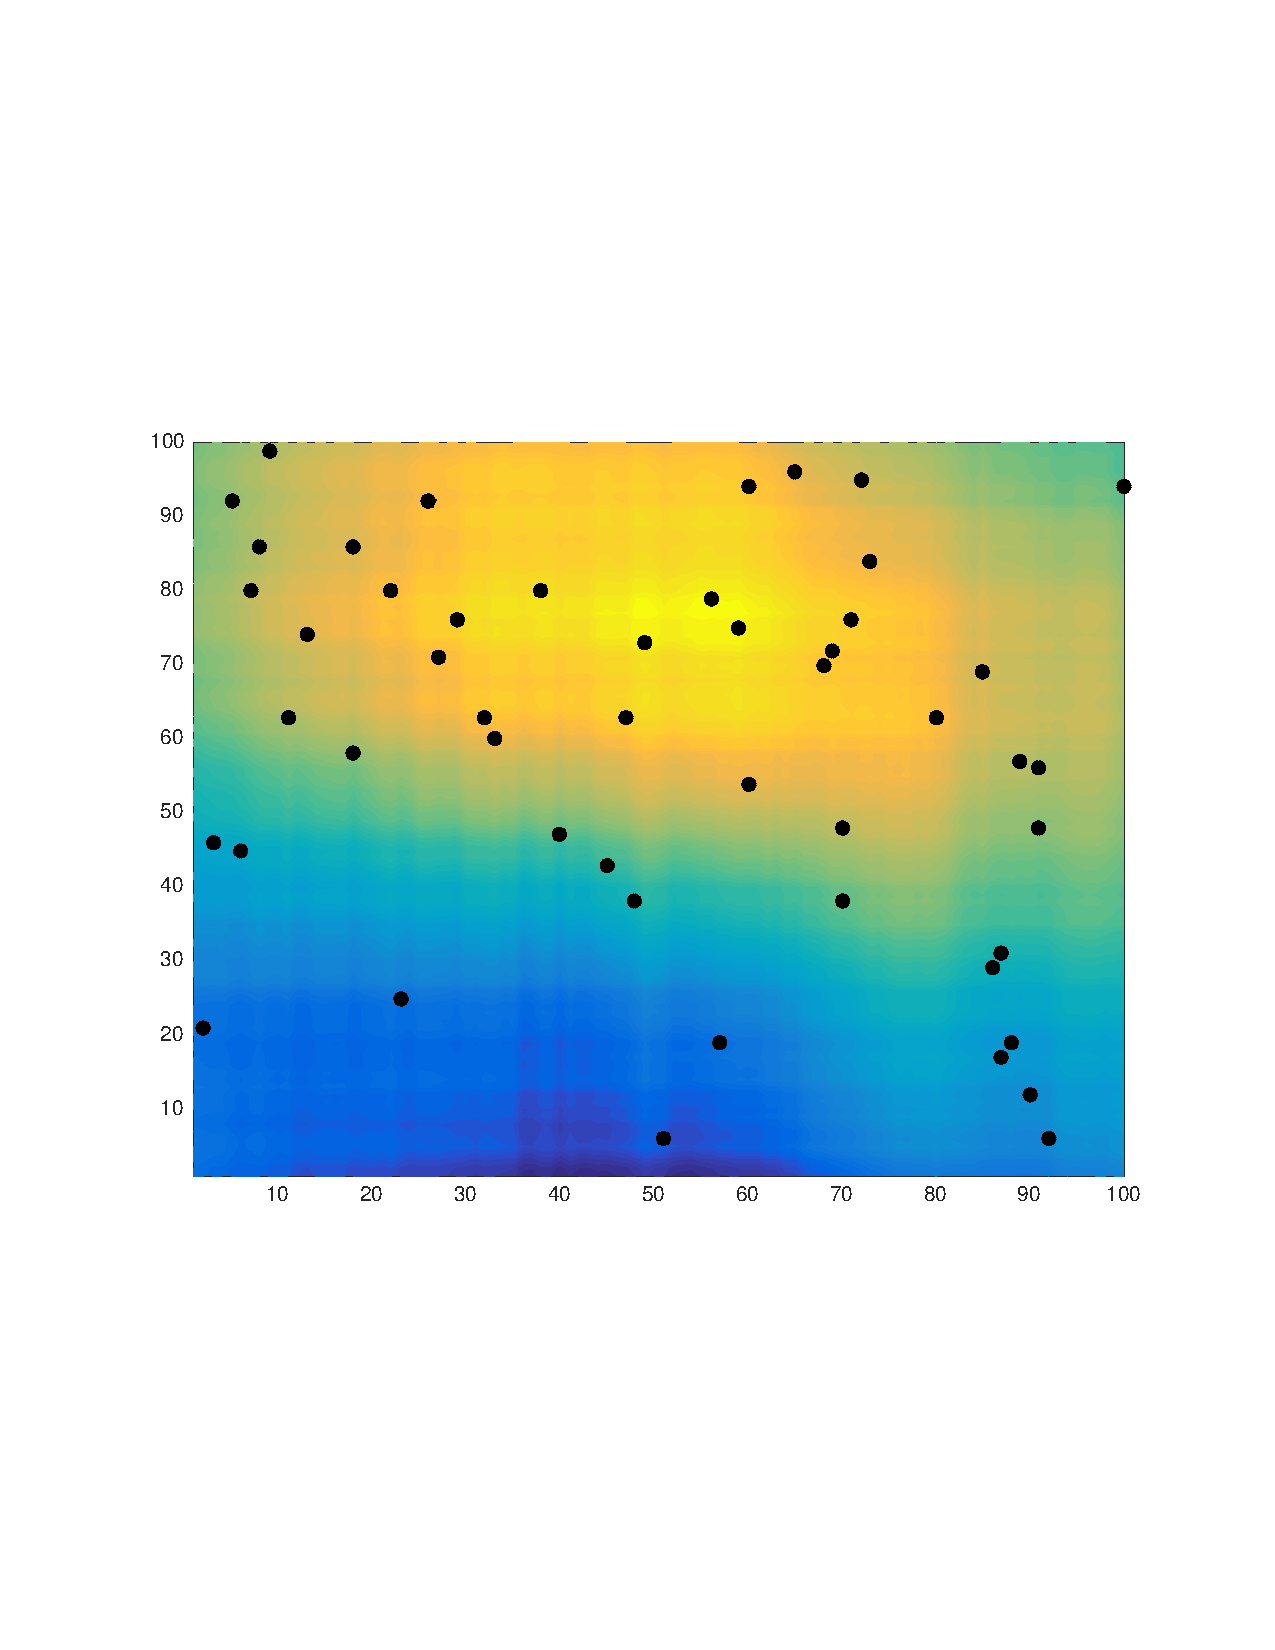
\includegraphics[width=\linewidth]{figures/sampled_generated_field.png}
        \captionsetup{skip=0.5\baselineskip,size=footnotesize}
        \caption{Sampled locations (50 points marked in black) of the previously generated geospatially autocorrelated field}
		\label{fig:sampled_field}
    \end{subfigure}%
    ~ 
    \begin{subfigure}[t]{0.5\textwidth}
        \centering
        \includegraphics[width=\linewidth]{figures/idw_predicted_field.png}
		\captionsetup{skip=0.5\baselineskip,size=footnotesize}
		\caption{An Inverse Distance Weighting generated predicted field ($p=3$). Generated from 50 randomly observed points.}
		\label{fig:idw_field}
    \end{subfigure}
    \captionsetup{skip=0.5\baselineskip,size=footnotesize}
    \caption{A randomly generated field where 50 observations were made (left), and an Inverted Distance Weighted Prediction (right) of that field from the marked observations.}
    \label{fig:idw_side_by_side}
\end{figure*}


\newpage

\section{Variography}
Variography is a set of procedures for examining and interpreting spacial dependence and geospatial autocorrelation in observed data. We would like to unravel the autocorrelation, or spatial dependence, of observed data to factor into a classical Inverse Distance Weighting, yielding a Best Linear Unbiased Predictor. The heart of variography is the Variogram Function, a function of quantified dependence for observed data separated at a given distance on the domain.

\subsection{The Semi-Variogram}
A Semi-Variogram is a function representing the variance of the observation value difference between two sampled locations that are some vector $\vect{h}$ apart \cite{matheron:geostat}.
\begin{equation}
	\gamma(\vect{h})=\frac{1}{2V}\iiint_V [f(\vect{x}+\vect{h})-f(\vect{x})]^2 \,dV \\
\end{equation}
This definition can be adapted to 2-Dimensional fields that are more appropriate for our purposes. For all sample locations $\vect{x}_{i}$, $\vect{x}_{j}$, that are $h=\|\vect{h}\|=\|\vect{x}_{i} - \vect{x}_{j} \|_{2}$, with respective observations $Z(\vect{x}_{i})$ and $Z(\vect{x}_{j})$, we will define an Empirical Variogram, a discrete 2-D semi-variogram, as \cite{cressie:spatial}:
\begin{equation} \label{eq:exp_var}
	2\hat{\gamma}(\vect{h}+\vect{\delta}) := \frac{1}{|N(\vect{h}+\vect{\delta})|}\sum\limits_{(i,j)\in N(\vect{h}+\vect{\delta})}|Z(\vect{x}_i) - Z(\vect{x}_j)|^2 % (Cressie 1993)
\end{equation}
where $\vect{\delta}=\begin{bmatrix}\pm\delta\\ \pm\delta\end{bmatrix}$.\\\\
where $N(\vect{h}+\vect{\delta})$ is the number of pairs of data locations that are vector distance $\vect{h}+\vect{\delta}$ apart ($\delta$ is a bound of ranges acceptable to "bin" alongside $\vect{h}$).
This function gives us an approximate factor of the variance between all points that are distance (or lag) $h$ apart.\cite{cressie:spatial}
\begin{figure}[H]
    \centering    
	\includegraphics[width=\linewidth]{figures/exp_variogram.png}
	\captionsetup{skip=0.5\baselineskip,size=footnotesize}
	\caption{An experimental variogram generated using Equation \ref{eq:exp_var} ($\delta=0$) in \textit{MATLAB}}
	\label{fig:exp_var}
\end{figure}

\subsection{The Variogram - Fitting A Semi-Variogram Using Least Squares}
A Variogram, which is intended to be a continuous function, yields a variance between two observations $Z(\vect{x}_{i})$, $Z(\vect{x}_{j})$ at a distance $h$ apart, as:
\begin{equation}
	2\gamma(\vect{x}_i, \vect{x}_j)= \text{var} (Z(\vect{x}_{i}) - Z(\vect{x}_{j}))=E[( (Z(\vect{x}_{i}) - \bar{Z} ) - (Z(\vect{x}_{j}) - \bar{Z} ))^2]
\end{equation}

Because it is infeasible and likely impossible to estimate an observation value at each possible point to compute a total variogram, we will fit our discrete empirical variogram using a least squares fit. This approach will allow us to approximate $\frac{1}{2}\gamma(h)$ for all possible $h$.
\begin{figure}[H]
    \centering    
	\includegraphics[width=\linewidth]{figures/fit_exp_variogram.png}
	\captionsetup{skip=0.5\baselineskip,size=footnotesize}
	\caption{An second degree least-squares fit of the experimental variogram in Figure \ref{fig:exp_var}}
	\label{fig:fit_exp_var}
\end{figure}

\subsection{Fitting a Statistical Kernel Model for the Variogram}
range, kernel, sill -- gaussian, exp, spherical
% TODO write this
\begin{figure}[H]
    \centering    
	\includegraphics[width=\linewidth]{figures/fit_kern_comp.png}
	\captionsetup{skip=0.5\baselineskip,size=footnotesize}
	\caption{A comparison of the Gaussian Kernel and the Spherical Kernel fit to the data previously sampled}
	\label{fig:kern_fit}
\end{figure}
\subsection{Covariance-Variance Matrix}

\section{The Kriging Method}
\subsection{Exploiting Geospatial Autocorrelation}
\subsection{The Kriging Formula - A Best Linear Unbiased Predictor}

\section{Natural Neighbor Selection}
\subsection{Finding Natural Neighbors}

\section{Graph Construction}
\subsection{Vertices and Edges}
\subsection{Path Problems}
\subsubsection{Optimizing a Route}

\part{Efficient Interpolation}

\chapter{Introduction}
There currently exists no consumer-level UAV system that can autonomously scan a perimeter of area to quickly map an unknown field. Due to the benefits of the solution to the problem, in terms of scientific research and benefit to fire fighting, I believe that designing a modified mathematical statistical interpolation method could make this system possible. Using a modified Kriging Method and a custom autonomous pod-UAV simulation, I would like to demonstrate that the system is possible, and could also benefit a variety of civil servants and scientists. We will, in this chapter, develop the tools and understanding of a method for interpolating data autonomously from just a few measured positions.

\section{Kriging Prediction}
It can be impossible to scan every square unit of area in a field, even with UAVs. Depending on the size of the map, it can often be most beneficial, in the interest of time flying above an area, to get a good enough prediction of the status of a field based off of a limited number of samples.\\
The Universal Kriging Method, also known as the Wiener–Kolmogorov prediction, is a geostatistical Gaussian process interpolation method historically used in fields varying from natural resource location prediction for mining to real estate value appraisals.\\

Using the Kriging method, the unknown prediction of interest at point $s_{0}$ is achieved via:
\begin{equation}
\widetilde{Z}(s_{0})=\mathlarger{\sum\limits_{i=1}^{n}\lambda_{i}Z(s_{i})}
\end{equation}
where $\lambda_{i}$ is the Kriging weight associated with the sampled point at $Z(s_{i})$.

The Kriging method fits values to the $\lambda_{i}$ weights using information interpreted from the field as data comes into the system. 

\subsection{Variography in Kriging Weight Selection}
%% add more
The factors that play into the calculations of these weights come from the variances of disjoint points sampled in the fields as well as factors inversely proportional to the square distances of the point in question and all other points sampled. Hence, the method also provides a variogram (a continuous approximation of variances between any given point in the prediction area and another point) with its prediction. The variogram provides what could be used as a measure of confidence in the Kriging prediction. This comes from the fact that the fields in question contain points of interest that are geospatially autocorrelated. 

\subsection{Semi-Variogram}
Kriging finds a continuous variogram by computing a discrete variogram function, a \textit{Semi-Variogram}, from points it has actually sampled

\begin{equation}
\hat{\gamma}({\bf{h}})=\dfrac{1}{2N({\bf{h}})}\sum_{i=1}^{N({\bf{h}})}\Big[Z(s_{i})-Z(s_{i}+{\bf{h}})\Big]^{2}
\end{equation}
Where $N({\bf{h}})$ is the number of pairs of data locations that are vector ${\bf{h}}$ apart.

\subsection{Variogram}
The discrete function is then fit by a least squares to a continuous variogram that can be sampled at each point in question.
% conveyed information

% fit to different kernels
\subsubsection{Gaussian (Normal) Kernel}
\subsubsection{Spherical Kernel}
\subsubsection{Exponential Kernel}
\subsubsection{Other Kernels}

\subsection{Choosing Kriging Weights}
% inverse distances and variances

\subsection{Measuring Prediction Confidence}
% MSRE

\subsection{Drawbacks To The Kriging Method}
Although the method is optimal for data with no trends or drift, the use of the unmodified Kriging Method technique has the drawback of being computationally intensive and slow to compute in a live and timely manner. This is due to the multiple matrix inversions and least squares fittings required to calculate the weights of the interpolation from the continuous variograms. It would be desired, in the case of autonomous UAVs that must constantly steer themselves in the best direction, to quickly calculate probabilities and variances. We will further discuss methods of efficient interpolation using the Universal Kriging Method.


\section{Natural Neighbor Selection}
\subsection{Voronoi Tessellations}

\part{Autonomous Path Finding}
We know for a geospatially autocorrelated field there is a stochastic process underlying in the data we would like to predict, and therefore could interpolate further based off of the variances of two disjoint points in the field. The variances, from samples collected in the scanning process which factor into our variogram, then become our relative confidence scores of predictions in our field in question. The values in the variogram are what will be used to terminate the interpolation when a level of least-confidence in total prediction is achieved, and what will dictate the future scan locations for a UAV or a pod of UAVs.
\subsection{Constructing a Confidence Graph}
\subsection{Confidence Optimized Path Finding}

\chapter{Previous Work}
Some other research was once performed.

\part{Can it fly?}
\chapter{Introduction}

\section{Custom Simulation}
\subsection{Flying Engine}
\subsubsection{Plot Drawing}
\subsubsection{Way-point Selection}

\section{FastPAS}
\subsection{The Algorithm}
\subsection{Simulating It}

\section{Other Uses}
% real estate
% crypto price pred.
% gentrify

\chapter{Results}

\chapter{Conclusion}
The method has proven to be a powerful interpolation method in simulations for simulated fields. The Kriging method has proven to be a working aerial mapping technique that provides a robust model for predictions and confidence scores. The goal of this thesis will be to design the algorithm for use with a pod of autonomous UAVs. A modified technique will have to first be developed to reduce the computational complexity of the algorithm by autonomously selecting optimal neighborhoods of sub-areas to run the method on.\\
Once the new method has been developed, an accurate simulation demonstrating its effectiveness and potential to be used in a real pod of UAVs will then be created and demonstrated. 
If time and resources are available, the algorithm will be ported to a real pod of UAVs to accomplish the task of autonomous scanning using thermal imaging (via infrared sensors). Tests will be conducted to prove the effectiveness and time efficiency of the newly developed algorithm.

\nocite{*}
\bibliographystyle{plain}
\bibliography{yonan_cmpe_msc_thesis}

\appendix
\chapter{Ancillary Material}

\end{document}
